\chapter{State of the Art}%
\label{chapter:State of the Art}

\begin{introduction}
This chapter will provide a comprehensive review of current \ac{5G} and Wi-Fi integration efforts, existing authentication mechanisms, and challenges in device identification. It will also explore recent developments and proposed solutions in the field, setting the context for our research.
\end{introduction}

\section{\acs{5G} Network Architecture}

\ac{5G} network represent a major shift from previous version in the sense that it is a \ac{SBA} which incorporates \ac{NFV} and \ac{SDN} technology. These changes allow for seperation between \ac{UP} and \ac{CP}, improving scalability, and flexibility of deployments, but most importantly, it allows for a unified authentication framework.~\cite{23.501-p56}

\subsection{Why \ac{4G} need improved security?}

Each generation of cellular networks has defined at least one new authentication method. For example, \ac{4G} introduced EPS-AKA, and 5G introduced three authentication methods: \ac{5G-AKA}, \ac{EAP-AKA’}, and \ac{EAP-TLS}.

% !!! One of the problems is the USIM is expected ||
From the point of view of authentication, a cellular network consists of three main components: \acp{UE}, a \ac{SN}, and a \ac{HN}. Each \ac{UE} is expected to possesses a \ac{USIM} storing a cryptographic key, shared with the home network. In 4G networks, the serving network includes equipment like \acp{eNodeB} base stations, and  \acp{MMe} that manage connections. The \ac{UE} connects to this network through radio signals. The home network stores user information in a database called the \ac{HSS}, which handles authentication. Both networks communicate over an IP-based system, and all the main components working together form the \ac{EPS}.~\cite{cbl-comp-4g-5g-p3}

In \ac{4G} \ac{EPS-AKA}, there are two significant flaws. First, during the initial stage of the authentication process, the \ac{UE} must transmit its identity, specifically its \ac{IMSI}, to the serving network. This identity is sent over the radio network without encryption, exposing it to potential interception~\cite{cbl-comp-4g-5g-p3}. Second, during the authentication decision, the home network may provide an \ac{AV}, but this value is not directly included in the decision-making process, which is instead handled solely by the serving network~\cite{cbl-comp-4g-5g-p4}.

\begin{figure}[htbp]
    \centering
    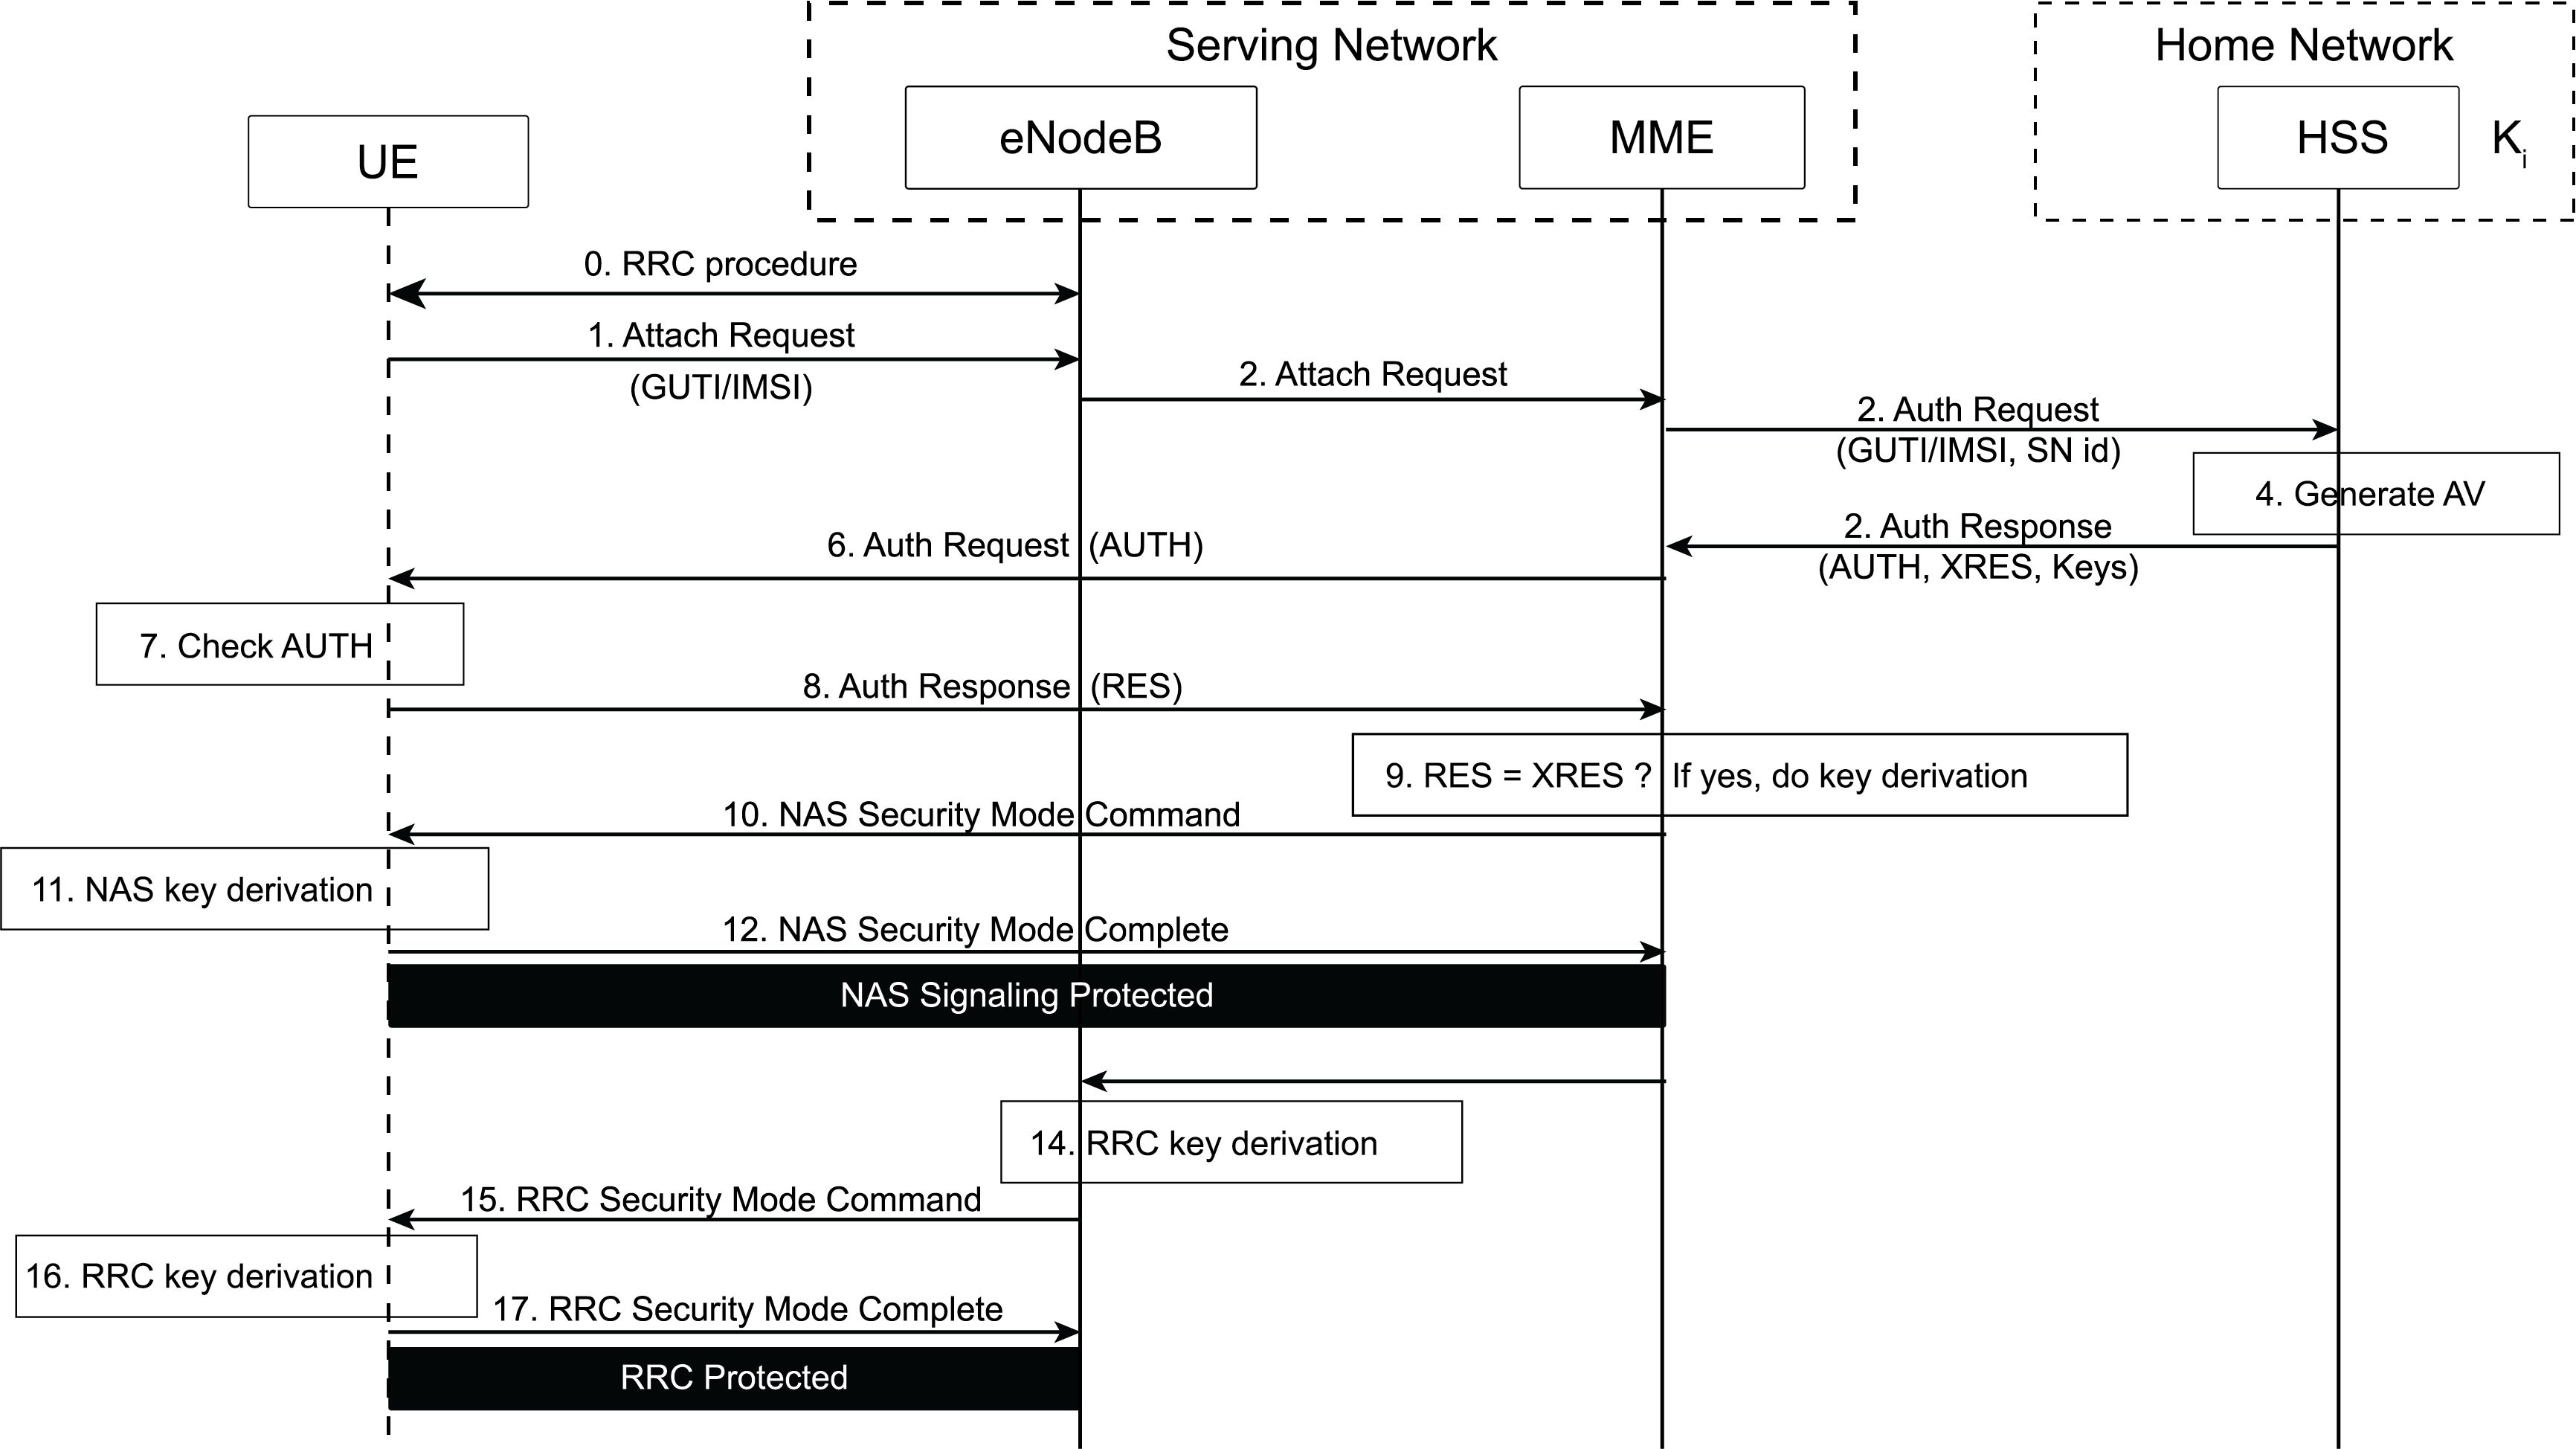
\includegraphics[width=0.8\textwidth]{figs/4g-authentication-flow.png}
    \caption{\ac{4G} Authentication Procedure}
    \label{fig:single}
\end{figure}

\subsection{\ac{5G} Security Framework}

\subsection{Support for Non-3GPP Access}

\ac{3GPP} refers to the standards developed for mobile networks, including \ac{3G}, \ac{4G}, and \ac{5G}. These are cellular technologies used by mobile carriers to provide network services. Non-\ac{3GPP} refers to other access technologies not standardized by \ac{3GPP} but still capable of integrating with \ac{3GPP} networks, such as Wi-Fi or satellite networks. These networks can provide connectivity, but following a different standards (e.g., IEEE for Wi-Fi).

In \ac{3GPP} architecture, trusted and untrusted refer to the way a non-\ac{3GPP} network (such as Wi-Fi) connects to the mobile core network. A trusted access network is a network that has been verified and trusted by the mobile operator. It connects directly to the core network using secure protocols and behaves similarly to \ac{3GPP} networks. For example, a mobile operator’s managed Wi-Fi network might be treated as trusted, while something like a public Wi-Fi hotspot managed by another provider may be considered as untrusted as it does not meet the same standards.

\section{Wi-Fi Integration Challenges}

\section{Authentication and Identity Management in \ac{5G}}

\section{Current Solutions and Proposals}